%% ****** Start of file apstemplate.tex ****** %
%%
%%
%%   This file is part of the APS files in the REVTeX 4 distribution.
%%   Version 4.1r of REVTeX, August 2010
%%
%%
%%   Copyright (c) 2001, 2009, 2010 The American Physical Society.
%%
%%   See the REVTeX 4 README file for restrictions and more information.
%%
%
% This is a template for producing manuscripts for use with REVTEX 4.0
% Copy this file to another name and then work on that file.
% That way, you always have this original template file to use.
%
% Group addresses by affiliation; use superscriptaddress for long
% author lists, or if there are many overlapping affiliations.
% For Phys. Rev. appearance, change preprint to twocolumn.
% Choose pra, prb, prc, prd, pre, prl, prstab, prstper, or rmp for journal
%  Add 'draft' option to mark overfull boxes with black boxes
%  Add 'showpacs' option to make PACS codes appear
%  Add 'showkeys' option to make keywords appear

\documentclass[aps,prl,groupedaddress,twocolumn]{revtex4-1}
%\documentclass[aps,prl,preprint,superscriptaddress]{revtex4-1}
%\documentclass[aps,prl,reprint,groupedaddress]{revtex4-1}

\usepackage{graphicx}
\usepackage{epsfig}
\usepackage{comment}
\usepackage{amsmath}
\usepackage{siunitx}

% You should use BibTeX and apsrev.bst for references
% Choosing a journal automatically selects the correct APS
% BibTeX style file (bst file), so only uncomment the line
% below if necessary.
%\bibliographystyle{apsrev4-1}

\begin{document}

% Use the \preprint command to place your local institutional report
% number in the upper righthand corner of the title page in preprint mode.
% Multiple \preprint commands are allowed.
% Use the 'preprintnumbers' class option to override journal defaults
% to display numbers if necessary
%\preprint{}

%Title of paper
\title{Catalytic Activity of Metallic vs. Oxidized Pt(110)}

% repeat the \author .. \affiliation  etc. as needed
% \email, \thanks, \homepage, \altaffiliation all apply to the current
% author. Explanatory text should go in the []'s, actual e-mail
% address or url should go in the {}'s for \email and \homepage.
% Please use the appropriate macro foreach each type of information

% \affiliation command applies to all authors since the last
% \affiliation command. The \affiliation command should follow the
% other information
% \affiliation can be followed by \email, \homepage, \thanks as well.
\author{Lassi Linnala}
\email[]{lassi.linnala.515@student.lu.se}
%\homepage[]{Your web page}
%\thanks{}
%\altaffiliation{}
\affiliation{Lund University}

%Collaboration name if desired (requires use of superscriptaddress
%option in \documentclass). \noaffiliation is required (may also be
%used with the \author command).
%\collaboration can be followed by \email, \homepage, \thanks as well.
%\collaboration{}
%\noaffiliation

\date{\today}

\begin{abstract}
Catalysis plays an important role in many places, such as in the battle against climate change, and it has been extensively studied within surface science community. Despite of this extensive research, there has a been a long disagreement on the active phase of Pt group metals for catalytic CO oxidation.  In this paper, I try to resolve this disagreement, by studying the deactivation of catalytic CO oxidation instead of the activation, at realistic pressures on an oxidized Pt(110). My mass spectrometry and surface x-ray diffraction studies reveal that the oxide formed on Pt(110) single crystal is at least as active as its metallic surface, which paves the way towards more fundamental understanding of catalytic reactions.

%Summarize the first three paragraphs in the introduction and each paragraph in the conclusions with one sentence each. Define the topic. Define the gap in the existing knowledge. Describe how you have filled this gap. Summarize your main conclusions. Why is this important and how can it change the world?
\end{abstract}

% insert suggested PACS numbers in braces on next line
% \pacs{}
% insert suggested keywords - APS authors don't need to do this
%\keywords{}

%\maketitle must follow title, authors, abstract, \pacs, and \keywords
\maketitle

% body of paper here - Use proper section commands
% References should be done using the \cite, \ref, and \label commands
%\section{}
% Put \label in argument of \section for cross-referencing

\section{Introduction}\label{intro}
Catalysis plays an important role in many areas, for example, in reducing the emission of greenhouse gases. Therefore, gaining a fundamental understanding of catalytic reactions have been a major part of research within surface science for few decades. In catalysis, the rate of a certain chemical reaction is increased by introducing a catalyst, for example, using a platinium group metals to oxidize CO into CO$_2$, as commonly done in car catalytic converters. Furthermore, due to the simplicity and relevance for the industry, this CO oxidation has also been a very common model for catalysis research. 

Typically, surface science studies have necessarily been perfomed in an ultra-high vacuum environment (UHV), but in recent years a lot of this research has shifted towards more realistic conditions. However, operating in an UHV has been studied to have a significant impact on the catalytic reactions \cite{pressure}, and therefore, being able to narrow down this pressure gap has been very important for real world applications of catalysis. Several studies of CO oxidation Pt group metals have already been reported at realistic pressures \cite{1,2,3}, but yet there still is no complete agreement on the active phase of this oxidation. 

A high pressure surface x-ray diffraction (SXRD) study by Ackermann et al.,\cite{Ackermann} showed that the oxides formed on Pt(110) are significantly more active than the metallic surface. However, based on their experimental method of studying the activation of the catalytic CO oxidation, it is cannot be clearly distinguished whether the oxide is more active or if the oxide is actually formed as a result of the high activity of the metal. In a more recent SXRD study by Gustafson et al., \cite{Gustafson}, where the deactivation of the CO oxidiations was studied instead of the activation, it could be distinguished that the metallic surface of Rh(111) is more active than the surface oxide, while for Pd(100) the different oxides formed varied in activity.

In this paper, I present a SXRD and mass spectrometry (MS) study of the catalytic oxidation of CO on Pt(110) single crystal surface under realistic pressures, with an aim to find out whether the metallic Pt(110) surface is more active than the oxide formed on it. The experimental methdology follows the deactivation of the catalytic reaction rather than the activation, very similar as in \cite{Gustafson}. 

By studying the deactivation, the oxidized sample is initially at high temperature, with activity such that the reaction is limited by the transport of CO on to the surface, i.e., the reaction will be mass transfer limited (MTL). Slowly lowering the temperature decreases the activity, which then reduces the oxide coverage, exposing the metallic surface depending on its activity respect to the oxide. Going to low enough temperatures, the activity becomes so small that the surface will become covered by CO, which is inert, and therefore results in a sudden drop of the activity. This point is known as the extinction. From this deactivation experiment, two cases can be easily distinguished. If the oxide is less active than the metal, the oxide coverage will gradually decrease exposing more of the higher activity metal maintaining the reaction in MTL, until the temperature reaches the point of extinction. If the oxide is at least as active as the metal, the oxide coverage will remain almost unvaried until the extinction, where it abruptly disappears.






%The first paragraph (5-10 lines) shall define the broad topic of the paper. For instance, if the topic is catalysis, define what catalysis is and why it is important. If the paper concerns a certain kind of catalysis, introduce this as well. asdf

%The second paragraph (10-20 lines) defines a lack in the present knowledge. For instance, the active phase for CO oxidation is not well known although it has been studied very much. Discuss what others have done in order to fill this knowledge gap. Explain why this is not enough. (Still do not mention what you have done.) (This paragraph may be split in two.)

%The third paragraph (5-10 lines) explains what you have done in order to fill the knowledge gap from the previous paragraph. “In order to fill this knowledge gap, we have…” This is the first time (except for the abstract) you mention what you have done.

%The fourth paragraph (5-10 lines) previews the rest of the paper. Discuss what you have found (you can, but do not have to, reveal the main results here) and why this is important for the future. (The third and fourth paragraphs may be combined to one.)

\section{Materials and Methods}
All experiments were carried out at Lund University x-ray laboratory. A single crystal Pt(110) was placed in a high-vacuum (HV) environment. This HV was equipped with a gas flow system and a mass spectrometer, allowing for constant monitoring of the gasses. Prior to the experiment, the Pt(110) surface was cleaned by repeated cycles of sputtering with Ar$^+$ ions and annealing, until no impurities could be detected with SXRD. 

The clean bulk terminated Pt(110) surface exhibits a characteristic $(1\times2)$ missing-row reconstruction \cite{VLIEG_missing_row}, which was removed by exposing the surface to 100 mbar of CO at 600 K\cite{CO_induced_back_relax}. The CO flow was then cut down and the $(1\times1)$ Pt(110) was oxidized by exposure of 500 mbar of O$_2$ at 673 K for 20 minutes. After the pure oxygen exposure, CO was re-injected to the HV chamber in a gas mixture of O$_2$ and CO with flows of 20 mL/min and 1 mL/min, respectively, while maintaining the constant pressure at 500 mbar. 

A monochromatic Molybdenum K$_{\alpha}$ laboratory x-ray source with wavelength of $\lambda = 0.71$ Å and flux of $>25\times10^6$ photons/s was aligned with the sample, such that the x-rays were incident on the Pt(110) surface with a small angle of $\mu=0.2\si{\degree}$ for surface sensitivity.

To study the active phases of the CO oxidation on the Pt(110) surface, the deactivation of the reaction, with the above gas flow and pressure, was studied by slowly lowering the sample temperature in steps of: 300 K, 267 K, 233 K, 200 K, 167 K. Each temperature step was maintained for 1800 s, during which an integrated SXRD intensity was recorded. Gas analysis was constantly monitored with the mass spectrometer.
 
The scattered x-rays were detected using a 2D detector thats covers a large portion of the reciprocal space, which allows for simultaneous monitoring of the diffraction from both the substrate crystal truncation rod (CTR) and the oxide at $(h,k,l)=$ $(0,-1,l)$ and $(0,-1.42,l)$, respectively.








\begin{comment}
	All experiments were carried out in the Obelix UHV environment with base pressure of $10^{-10}$ mbar at Lund University. This environment consisted of a preparation chamber and an analysis chamber, where the latter is equipped with room temperature STM and LEED. The Ir(111) single crystal was cleaned by repeated cycles of annealing at 1400 K,  hot sputtering with 1 kV Ar$^+$ ions at 1000 K ($p=10^{-5}$ mbar, $HV = 650$ V, $I_{ems}= 10$ mA) and exposing to system to oxygen atmosphere of pressure $p=10^{-7}$ mbar at 800 K.
	
	\textbf{Growth hBN/Ir(111):} Prior to the hBN growth, the precursor borazine was purified by three cycles of freeze-pumb-thaw. The hBN monolayer was grown by CVD, exposing the Ir(111) substrate to 100 L of borazine ($p=10^{-6}$ Torr for 100 s) at 1250 K in the preparation chamber. The high quality of the grown hBN monolayer was verified with STM and LEED and is discussed in Sec. {\ref{hbn/ir(111)}}.
	
	\textbf{Growth Gr/hBN/Ir(111):} The electron beam from the filament, (I = 4 A and HV = 200 V), in the EAG technique was used to dissociate the hydrocarbons from the precursor molecule ethylene.
	Two doses, followed by step-wise annealing were characterized, namely: Dose 300 L ethylene ($p=10^{-6}$ Torr for 300 s at RT), anneal in steps of 773 K, 1073 K and 1273 K. Start over by cleaning the sample and growing hBN with the above recipe, then: Dose 6000 L ethylene ($p=10^{-5}$ Torr for 600 s at RT), anneal in steps of 773 K, 973 K, 1173 K and 1373 K. STM and LEED characterization were performed after every step. The temperatures were carefully measured using infrared pyrometer. This temperature evolution is discussed in Sec. {\ref{gr/hbn/ir(111)}}. Furthermore, the acquired STM and LEED images were processed and analyzed using ImageJ and Igor Pro softwares.
\end{comment}


%Where and how were the measurements/the study done? For instance, "The XPS experiments were done at beamline i311 at the MAX IV laboratory" [reference to paper about the experimental station]? Did you use any special equipment? Were there any special settings, such as photon energy, used throughout the study? Do not mention if it does not apply to all measurements. How were the data analysed? Is there anything special, such as choice of coordinate system, that the reader needs to know about in order to interpret the data in the paper?

%What kind of samples were used and how were they prepared?

%How were the measurements performed? Again, only discuss common features between all the reported measurements. "In order to investigate the deactivation of the catalyst, the activity was first started by heating the sample in the reaction gas mixture, after which the temperature was lowered slowly until deactivation." Since the gas mixtures were different in the different measurements, I do not mention them.

%Anything else that can be important for the outcome of the experiments, that is not obvious from the choice of method or setup? This section should provide enough information for someone who is familiar with the method to be able to judge the quality of the results.


\section{Results}
Figure \ref{fig1} shows the mass spectrometry and SXRD measurements during the cooling down of the oxidized Pt(110) single crystal, in a flow of 20 mL/min and 1 mL/min of O$_2$ and CO at 500 mbar, respectively. \ref{fig1}a shows the measured CO$_2$ mass spectrometer signal as a result of CO oxidation. At high temperatures, the reaction is MTL and the observed slight decrease of the signal with decreasing temperature is only due to degasing of the filament. Around 235 $\si{\degreeCelsius}$ the CO$_2$ mass spectrometer signal drops abruptly. This is the point of extinction, which occurs due to the surface becoming covered by CO, stopping the dissociative adsorption of O$_2$. 

Figure \ref{fig1}b shows the corresponding SXRD measurements of both the CTR (orange) and the oxide (blue). At high temperatures, the Pt(110) surface is largely oxidized, but after the extinction, diffraction from the oxide dissappears and the intensity of the CTR is increasesed in turn, i.e., the surface is now metallic. Because of the few data points, the decrease of the oxide seems gradual, but in reality is abrupt. As described in the introduction, since the CO oxidation activity, shown in a, does not increase when the surface becomes metallic and the drop of the oxide at the extinction is abrupt, the oxide is, therefore, at least as active as the metal.


%For each figure, describe in one sentence the general content of the figure. Then guide the reader through the data of the figure and introduce the different subfigures if there are any. This section is supposed to be objective, that is, you should report what is shown in the figure, but not more interpretation than necessary.

%"Figure 1 shows the deactivation of the CO oxidation reaction on the epitaxial bulk oxide on Pd(100) during a slow cooling process. The O$_2$:CO ratio was? Panel a shows the CO$_2$ RGA signal (blue), monitoring the catalytic activity, as well as the sample temperature (red). The constant CO$_2$ signal in the beginning shows that the catalytic reaction is active enough to be mass transfer limited, but after about 1700 s, the activity suddenly drops significantly. The temperature drops slightly at the same time, as expected since reaction is very exothermic. Figure 1b shows...  This shows that the Pd oxide is at least as active as the metallic surface."

\begin{figure}
%\includegraphics[width=8.5cm]{sxrd_final.png}
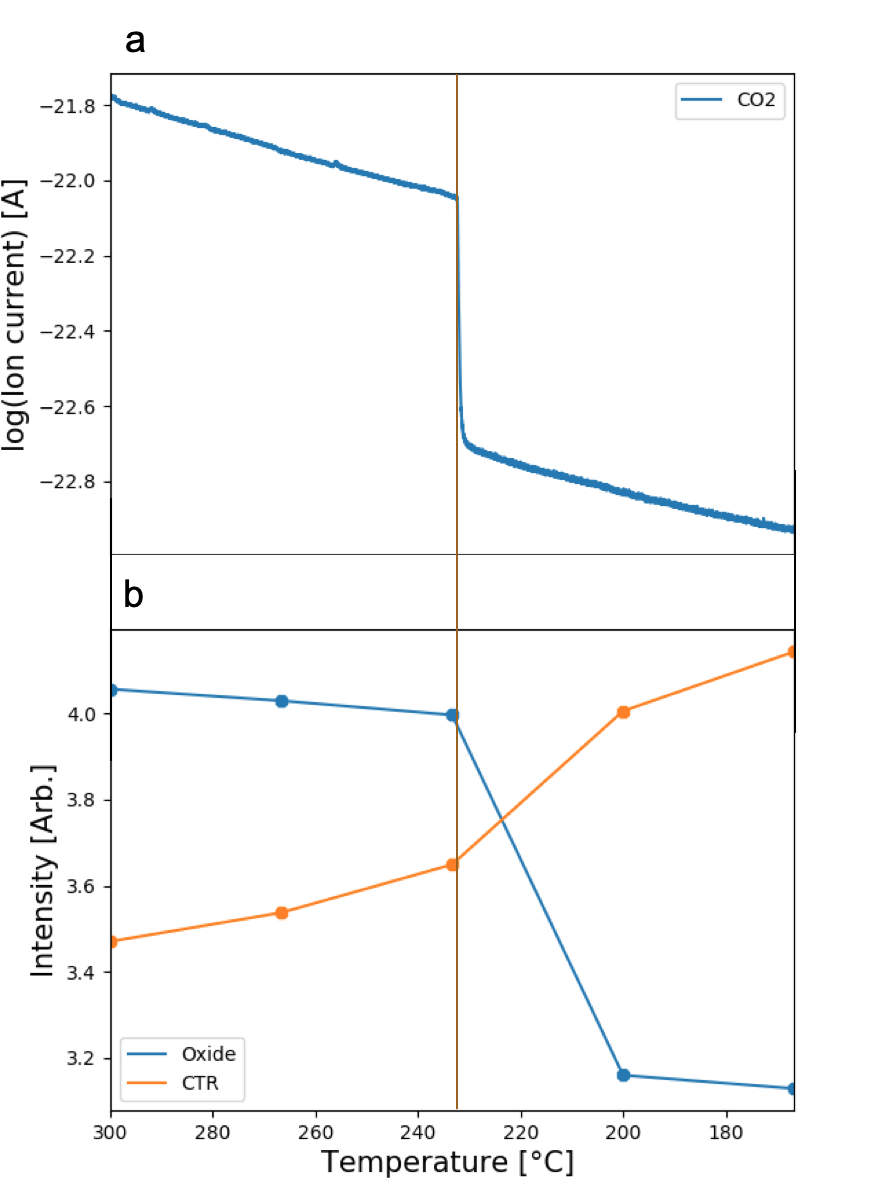
\includegraphics[width=8cm]{edited_1_fig.png}
%\includegraphics[width=8cm]{SXRD_with_pts.png}
\caption{\textbf{Mass spectrometer and SXRD measurement of deactivation of the CO oxidation.} (a) Measured CO$_2$ signal in the mass spectrometer. Activity declines steadily as a function of the sample temperature until extinction at around 235 $\si{\degreeCelsius}$. (b) SXRD intensity for both the oxide and the CTR with exposure time 1800 s between the data points. The oxide disappears abruptly from the surface at the extinction. The abrupt drop of the oxide at the extinction indicates that the oxide is at least as active as the metallic surface.}

%Describe the conditions for the measurements reported in the figure. Describe each of the panels and the data. Preferably, a basic interpretation of the data should be possible from only the figure and the caption. Still it should not be too long, so you have to make your own judgement on how much to include.
\label{fig1}
\end{figure}



\section{Discussion}
My results show that the oxide formed on Pt(110) stays until the activity drops, suggesting that the oxide is at least as active as the metallic surface. The present study, studying the deactivation, is not, however, able to distinguish whether the oxide is more active than the metal. 

At first sight, as already mentioned in the introduction, the SXRD study of the activation of the catalytic CO oxidation on Pt(110) in Ref.\cite{Ackermann} showed that the oxides on Pt(110) have significantly higher activity than the metal. However, as a consequence of studying the activation, it could not be clearly determined whether the oxides are more active, or if they rather are formed on Pt(110) as a result when the catalyst becomes active. 

In a similar SXRD study to Ref.\cite{Ackermann} for CO oxidation on Pt group metals, it could be distinguished that the Rh(111) surface is more active than the oxide, and for Pd(100), the thin oxide films are at least as active as the metal whereas thicker oxide films become less active \cite{Gustafson}. This distinction could easily be achieved by studying the deactivation instead of the activation, as also done in this paper. Therefore on this note, it can be argumented and verified that the oxide is at least as active as the metallic surface.


%Summarize the results in one sentence. Discuss for one paragraph how you interpret these data and the main conclusions. Now the discussion does not have to be as objective anymore, and you are allowed to speculate as long as you make this clear.

%Mention previous studies of the same or similar systems and how they agree or disagree with the results of this study. It has to be clear from the discussion that your results increase the knowledge in a useful way.

%\textit{Our results show that the reaction between CO and preadsorbed O happens at lower temperature on the stepped Rh(553) surface than on flat Rh(111). This is in agreement with the general assumption that the under-coordinated... \cite{Gustafson}, \cite{Ackermann}  }

\section{Conclusions}
In summary, this paper studied the active phase of Pt(110) single crystal for catalytic oxidation of CO with SXRD and MS. It was found that the oxides formed on Pt(110) are at least as active as the metallic surface. For Pt(110), this result resolves one of the long-standing debates concerning whether the oxides formed on Pt group metals are actually active, or if they are just formed as a result of the high activity. Futhermore, by studying the deactivation catalyst reaction instead of the activation, a better understanding of catalytic reactions under realistic pressures can be achieved. This information can be of use for the further development of important catalyst applications even outside CO oxidation, such as oxidizing methane.

%Summarize the results and discussion in one sentence. Try to generalize and discuss whether these results, in one way or another, can be valid for other similar, or not so similar, systems.
%Discuss how the results can be important. Will your results open up opportunities for further studies? Will they lead to the development of new devices? How will this change the world? Here you are free to speculate quite freely, as long as you are open with it. "This could potentially lead to the end of climate warming?" 


\section{Acknowledgments}
The author would like to thank Kim von Allmen for both performing and instructing this experiment, and Johan Gustafson for the feedback on writing this paper.

% Create the reference section using BibTeX:
\bibliography{References}

%ALTERNATIVE REFERENCE STYLE

% \begin{comment}
% \begin{thebibliography}{99}

% \bibitem{lundgren1}
% E. Lundgren, H. Over, \textit{In situ gas-surface interactions: Approaching realistic conditions.} J. Phys.: Condens. Matter \textbf{20} (2008) 180302.

% \end{thebibliography}
% \end{comment}


\end{document}
%
% ****** End of file apstemplate.tex ******

